\subsubsection{Scrapy}
\label{ss:scrapy}

\textbf{Scrapy} is a framework for large scale web scraping. It provides all the tools to efficiently extract data from websites, process it and store it in the appropriate structure and format. We decided to utilize this tool as it one of only scraping frameworks ready to be easily scalable and that is already split into independent modules.

The following Figure \ref{fig:scrapy-architecture} shows an overview of the Scrapy architecture with its components and an outline of the data flow that takes place inside the system (shown by the red arrows).

\begin{figure}[H]
	\centering
	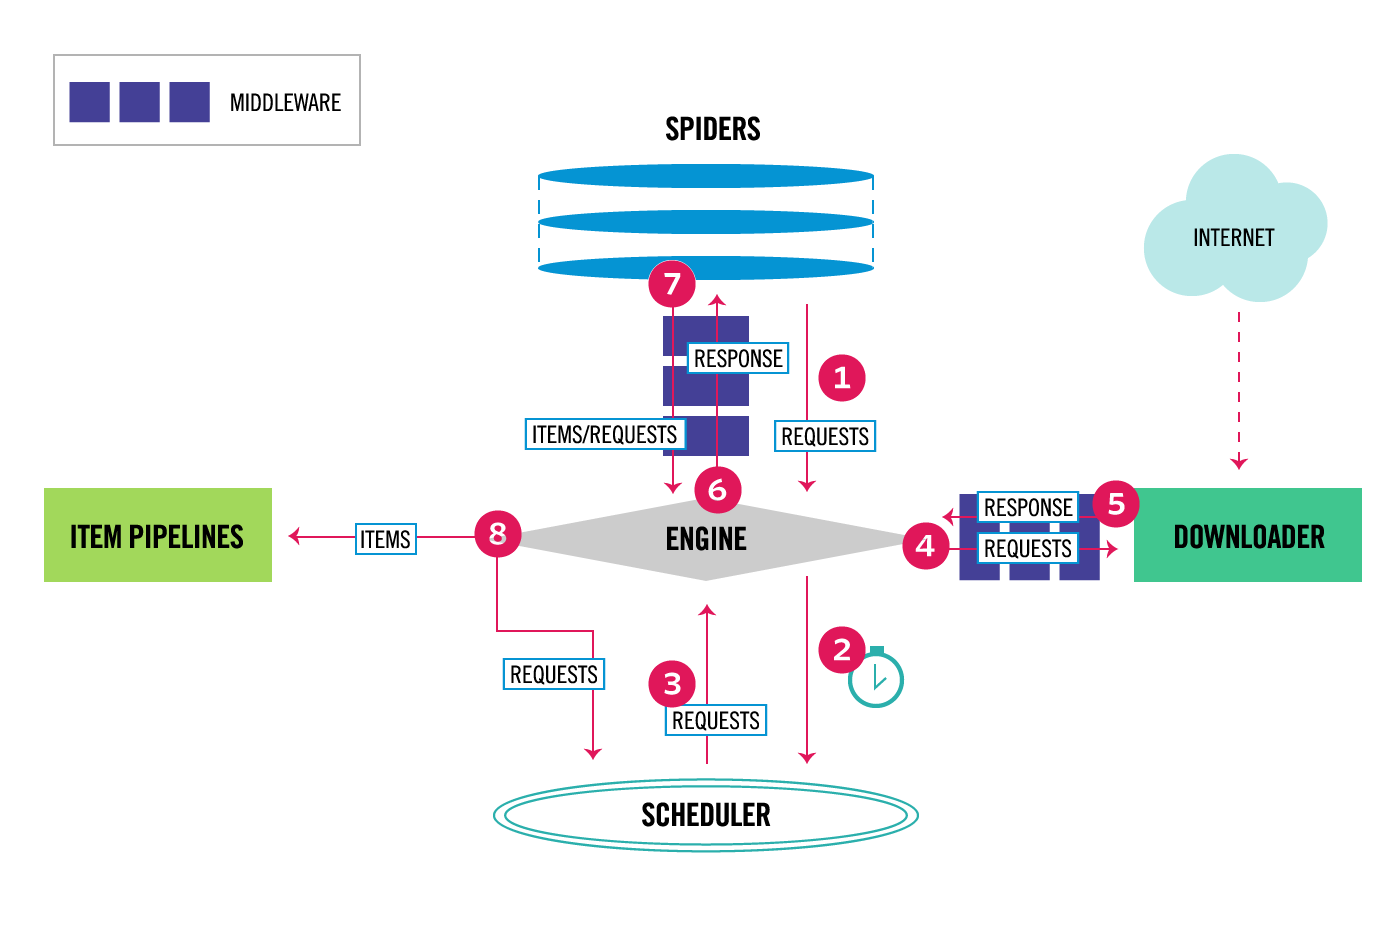
\includegraphics[width=1\linewidth]{Chapters/img/2_background/scrapy_architecture.png}
	\caption{Scrapy dataflow \cite{scrapy-architecture}}
	\label{fig:scrapy-architecture}
\end{figure}

First of all \textbf{Spiders}, the main workhorse of Scrapy, are the classes used to define the custom behaviour for parsing the page(s). Along with that, (1) they are also responsible for sending the requests to the scrapy Engine. The engine controls the data flow between all components of the framework and triggers events when certain actions occur. These initial request(s) are responsible for starting the scraping process.

(2) Those requests are then sent to the \textbf{Scheduler}, which is responsible for collecting and dispatching requests made by the spiders. This scheduler is necessary because scrapy follows asynchronous processing, so requests are made but the process doesn't wait for the responses and continues with further tasks. When a response arrives, the requesting process deals with it. (3) The requests are then dispatched by the scheduler to the engine for further processing.

(4) These requests are then sent to the \textbf{Downloader} going through the defined middlewares. At the downloader (5) the requested page is downloaded, which generates a response that is sent back to the engine. These downloader midlewares are usually used to process requests just before they are sent to the download, change received response before passing it to a spider or even silently drop requests.

(6) The engine sends the response from Downloader to the respective spider that generated the request through the Spider Middleware, the spider then processes the response by extracting information through the use of selectors, scrapy mechanisms to select HTML with XPath expressions, as explained before. This information is stored in items, usually defined as key-value pairs. The response may also generate further requests from that response, if needed, which are sent to the engine.

(8) The engine sends the extracted items to \textbf{Item Pipelines}. This pipeline components are Python classes that implements simple methods, where they receive a method and perform an action over it, deciding if the item should continue through the pipeline or be dropped and no longer processed. Being the most common uses data cleansing, validation or storage of the obtained item.

All of this process is repeated until no further requests are found in the Scheduler. One advantage of having the scheduler as an independent module is the possibility of using external tools to implement it, one of these tools is Redis which already has an external library ready to be implemented with Scrapy \footnote{\url{https://scrapy-redis.readthedocs.io/}}.

% -------------------------------------------- Redis 
\subsubsection{Redis}
\label{sss:redis}

%% -- Created: 12-10-20
%% -- Last edit: 05-07-21

Redis \footnote{\url{https://redis.io/}} is an open source, in-memory key-value data structure store, used as non-relation database, cache and message broker. Due to its low data structure complexity, Redis provides large performance advantages in comparison to relation databases mainly in speed, due to the fact that it is almost fully implemented in memory, and although its main purpose is for database implementations, it is widely used as a caching solution~\cite{9047417}. It supports replication to scale read performance, in-memory persistence, storage on disk, and client-side sharding to scale write performance. Data can be persisted either by periodically dumping the dataset to disk (snapshotting) or by appending each command to a disk-based log.

Redis stores data in key-value pairs, where a key has to be unique and always represented as a byte array independently of the content type. Values wise, it is limited to the following data structures: strings, hashes, lists, sets and sorted sets. For indexing, it attempts to create secondary indexes through the use of ZSET's, the redis implementation of sorted sets.

% -------------------------------------------- Selenium 
\subsubsection{Selenium}
\label{sss:selenium}

%% -- Created: 12-10-20
%% -- Last edit: 03-07-21

As stated previously some of the websites encountered had content load only through user interaction, as such it required a solution to automate this interaction. Selenium is one of the most common frameworks for this type of work. It is usually used as a portable framework for web application testing, with tools to automate and simulate human browing behaviour. Despite serving its major purpose, we decided to use it as a way to interact with our pages and force them to load so they could be scraped.

Using the Selenium WebDriver API in conjunction with a browser driver (such as ChromeDriver for the Google Chrome Browser) will act the same way as if a user manually opened up the browser. Because of this, loading and scraping web pages that use JavaScript to update the DOM no longer pose a challenge.

During use, selenium is controlled by either recording usage patterns within a browser or by programmatically driving it using its library methods.

\subsubsection{PostGIS/PostgreSQL}
\label{ss:postgis}

%% -- Created: 07-10-20
%% -- Last edit: 07-07-21

% Página 24 - https://run.unl.pt/bitstream/10362/2318/1/TGEO0003.pdf
% Página 52 - file:///home/leo/Downloads/TSIG0065.pdf

%PostGIS spatially enables PostgreSQL by addin support for geographic objects and thus, it can be used as a spatial database for GIS applications. It already supports several geometry types, topology, data validation, coordinate transformation, networks and routing analysis and \acrshort{api}s. Further deve

%Spatial databases are an extension of general purpose databases, which provide spatial indexing and support spatial queries. These features improve performance for geospatial applications. In this prototype, since 

Spatial databases extend general purpose databases by providing spatial indexing and support for spatial queries. They are able to store geographic objects in either vector or raster based formats, which allows effective and efficient management and organisation of geospatial data. Even though there are multiple solutions to save this type of data, we have chosen a technology we are already familiar with as a way to reduce labor and cut learning time.

PostgreSQL \footnote{\url{https://www.postgresql.org/}} is a powerful, open source object-relational database system with more than 15 years of active development. It runs on the major operation systems and has support for features such as foreign keys, joins, viewers, trigger, and stored procedures. PostGIS is a project which adds support for geographic objects in PostgreSQL, allowing it to be used as a spatial database for GIS. 

PostGIS \footnote{\url{https://postgis.net/}} is a popular choice given that is open software, it is kept up to date frequently and works well with the main GIS and Web GIS software.



%%%%%%%%%%% TECNLOGIAS DO CAPITULO MICROSERVICES

\subsubsection{Containerization}
\label{sss:containerization}
%% -- Created: 14-10-20
%% -- Last edit: 03-07-21

\paragraph{\textbf{Docker}}~\footnote{\url{https://www.docker.com/}} is a platform for developing, deploying and running applications within containers~\cite{docker-overview}. It uses a client-server architecture, where the docker client talks with the daemon (\textbf{dockerd}) responsible for building, running and distributing docker containers. The daemon listens for Docker \acrshort{api} requests and manages Docker objects such as images, containers, networks, and volumes. 

An image is a read-only template with instructions for creating docker containers, it is usually based on other images with additional customization. For example, an image may be based on an ubuntu image, but installs nginx and an application on top of it, as well as the configuration details needed to make the application run. This images are built with \textbf{Dockerfiles}, a file with a simple syntax for defining the steps needed to create the image and run it. 

The daemon is responsible for getting the images from local services such as Docker Registry, or public online registries such as Docker Hub via \acrlong{http} (\acrshort{http}).

\begin{figure}[h]
    \centering
    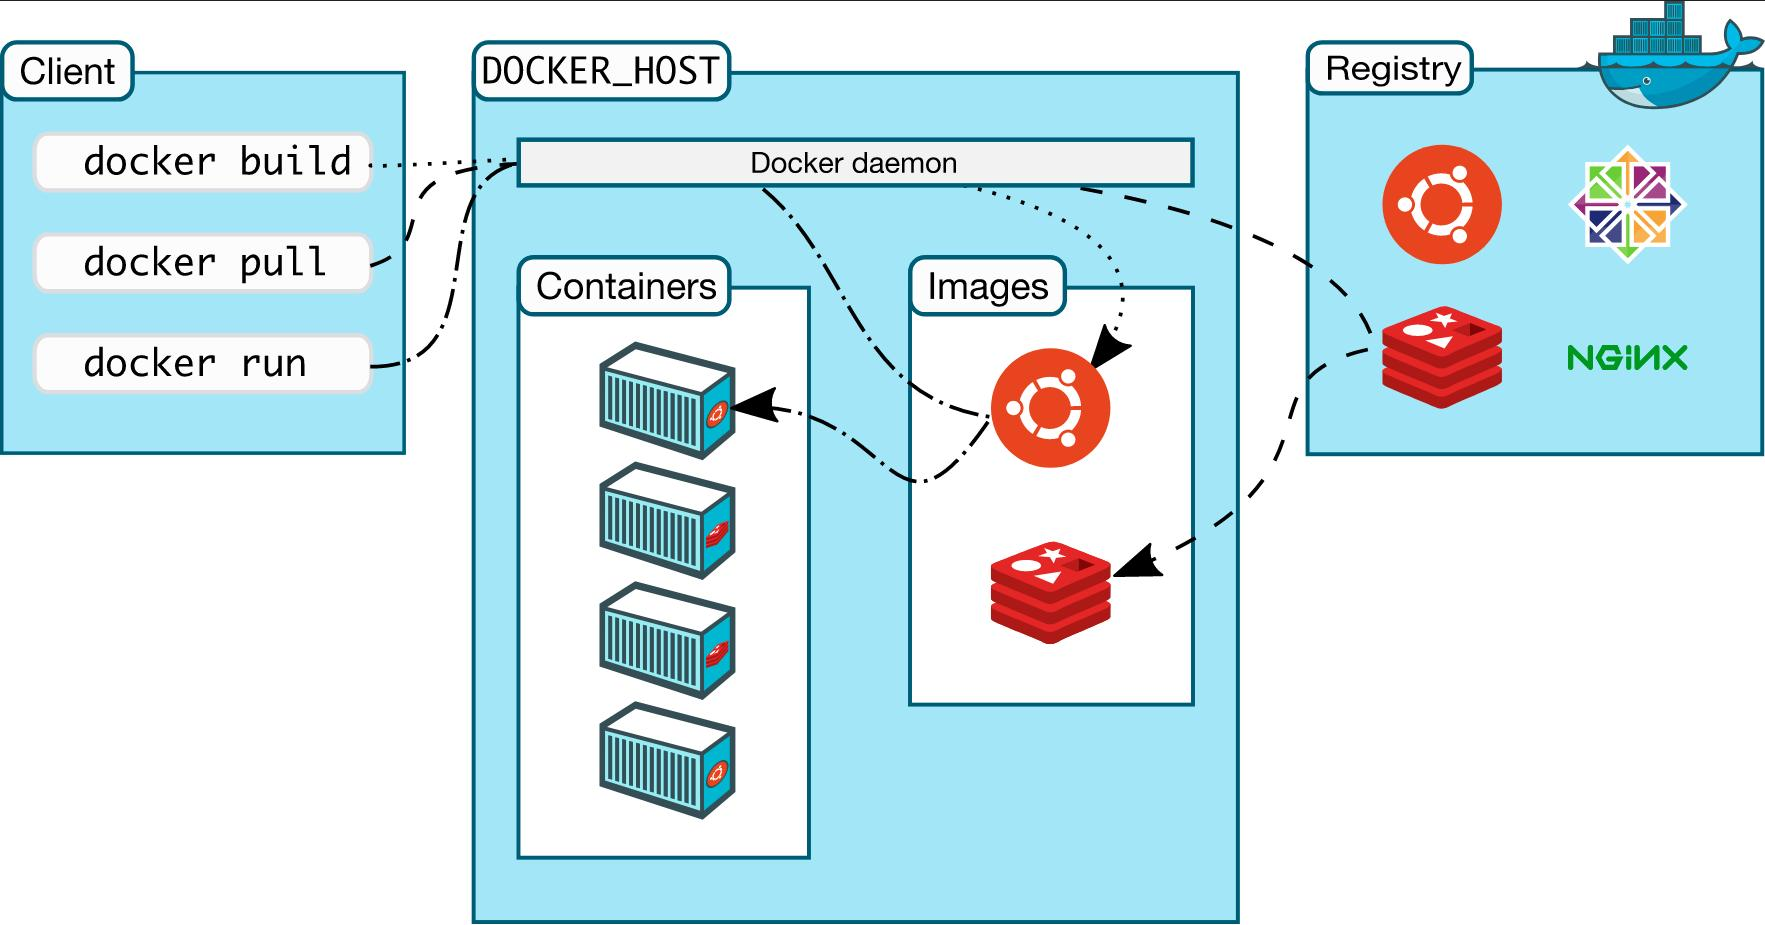
\includegraphics[width=1\textwidth,clip,trim=0 0 0 5]{Chapters/img/2_background/docker-architecture.jpg}
    \caption{Docker architecture~\cite{docker-overview}} 
    \label{fig:docker-architecture}
\end{figure}

The client, is the primary way that users can interact with Docker with commands such as \texttt{docker run}, which the client sends to dockerd, which carries them out. This client and daemon can run on the same system or remotely and they communicate using a \acrshort{rest} \acrshort{api}.

%Docker is a tool that can package software into containers that run reliably in any environment. A container is a standard unit of software that packages up code and all its dependencies so the application runs quickly and reliably from one computing environment to another. Meanwhile, a Docker container image is a lightweight, standalone, executable package of software that includes a snapshot of the software and all the necessary dependencies (code, runtime, system tools, system libraries and settings). This images are created from \textit{dockerfiles}, where the code instructs docker on how to build the image. This results in an imutable image that can be used to spin-up multiple containers.

%---------------------%------------- Docker Services -----------------------------
%\paragraph{Docker services}
%\label{par:docker-services}
%% -- Created: 03-07-21
%% -- Last edit: 03-07-21

In microservice based applications, a system is usually made up of different services such as: databases, \acrshort{http} servers, databases or any other type of executable program. Frequently a service is the image for a microservice within the context of some larger application.

When a service is created, it is specified which image to use, which commands to execute inside the running containers, and the following options:

\begin{itemize}
    \item The port that makes the service publicly available;
    \item The network the service should join;
    \item \acrshort{cpu} and \acrshort{ram} limits;
    \item Rolling update policy, which specifies how to update the services while avoid downtime;
    \item The number of wanted replicas.
\end{itemize}

Docker was chosen as it made containers easier and safer to deploy and use than previous approaches, in addition, Docker partnered with multiple companies such as Canonical, Google, Red Hat, and Parallels that brought standardization to containers. With all this components in mind, Docker, currently, does not have any rivals per se. 

%------------------------------------------%------------- Docker Swarm -----------------------------
\subsubsection{Orchestration}
\label{sss:backend-orchestration}

There are two main orchestration tools, Docker Swarm and Kubernetes, which we will now detail.

%\subsubsection{Docker Swarm}
%\label{sss:docker-swarm}
%% -- Created: 03-07-21
%% -- Last edit: 04-07-21

\paragraph{\textbf{Docker Swarm}} was released by Docker, and as such the deployment of this engine is greatly simplified and easily integrated with other components of the Docker environment. It provides a way to configure and manage containers, regardless of whether it's an individual container or a larger number of them. It helps ensure the cooperation of containers, as docker containers are designed for individual operation and cannot cooperate with each other on their own~\cite{docker-container-isolation}.

A swarm is a cluster of nodes, each of which can be of the \textbf{manager} or \textbf{worker} type. The manager nodes are responsible for the controlling the configuration and state of the swarm, being the only nodes capable of creating and distributing containers to workers, as well as allowing them to execute docker specific commands. While worker nodes have the sole purpose of executing containers, under the orders of the control node. As they are working they send status updates of the task being performed.

Some advantages and features available in Docker Swarm:

\begin{itemize}
    \item \textbf{Docker engine integration:} as mentioned previously it was released by docker, as such it has access to all docker features, allowing clusters to be created and managed directly through the Docker Command Line, without requiring any aditional software.
    \item \textbf{Scalability}: It can create and remove tasks, automatically, according to the number of tasks defined in the configuration file, keeping the container environment in the desired state;
    \item \textbf{Declarative design:} it provides a declarative approach to defining services, which allows the definition of desired state and type of various services;
    \item \textbf{Service discovery:} Swarm includes a \acrlong{dns} (\acrshort{dns}), as such the swarms allows containers to communicate with each other through their service name;
    \item \textbf{Security:} all nodes in the cluster can use authentication and encryption mechanisms to secure communications between the other nodes in the cluster. It uses \acrlong{tls} (\acrshort{tls}) certificates, which can either be self-signer or signed through a \acrlong{ca} (\acrshort{ca}).
    \item \textbf{State preservation:} the control node keeps track of the state, and if necessary, corrects the problem which caused to state to change. As an example, if we declare that service is made of 1 replica and this replica dies, the swarm executes it once again to preserve the required state;
    \item \textbf{Load Balancing:} Docker swarm allows for external load balancing (by exposing the service ports) or internal load balancing;
    \item \textbf{Update rollback:} Restore points are created for each update, in case a service update is not successful, it is possible to return to the previous version.
\end{itemize}

%------------------------------------------%------------- Kubernetes -------------------------------
%\subsubsection{Kubernetes}
%\label{sss:kubernetes}
%% -- Created: 14-10-20
%% -- Last edit: 03-07-21

\paragraph{\textbf{\acrlong{k8s}}}, also known as \acrshort{k8s}, is one of the available tools, and the most popular, for container orchestration. It was initially developed by Google, but later entrusted to the Cloud Native Computing Foundation (CNCF), which is run by the Linux Foundation. Kubernetes is a very complex system to automate the deployment, planning and scaling of applications packaged in Docker containers. 

%In a real world scenario such as a stock trading app, while the market is closed, the request volume tends to be lower which in turn requires a lower number of resources, system wise. However, as soon as the market opens it needs to handle millions of trades per second, kubernetes is the tool responsible for orchestrating the infrastructure necessary to deal with this change, which it does by scaling up or down the containers, and knows how to replace them automatically in case of failure.

Kubernetes is usually deployed in a cluster, and brain of this cluster is known as the \textbf{control-plane} which exposes an internal and external server API used to manage the cluster. For storage, it uses a key-value database called \textbf{etcd}, which stores important information on how to run the cluster. Per cluster there is at least one or more \textbf{worker nodes} (machines), and each of these machines runs \textbf{kubelet}, a small application that allows the nodes to communicate back to the control-plane. 

In each node, there can be many pods, which is the smallest possible deployable instance in kubernetes. Each pod consists of one or more containers, with shared network, storage and instructions on how to run containers. Containers in the same pod share IP addresses, a port space and can find each other via localhost.

When pods malfunction and are destroyed, they are not resurrected. Specifically, \textbf{ReplicationControllers} are designed to create and delete pods dynamically when, for example, commencing rolling updates or scaling the deployment up or down. This replica sets keep multiples pods or containers running and ready to be used at any time, with their network, secrets, storage, etc... automatically configured. Allowing the system to obtain an higher availability.

All of this can be controlled in an imperative or declarative way. The latter is done with the help of objects made in YAML, which define the \textbf{desired state} of the cluster (selecting docker images, ports to export, mounting volumes, etc...). This definitions help provision and scale containers automatically ensuring they are always up, running and healthy.

For communication \textbf{services} can be used, the basic idea is to define a policy to gain access to the pods. They take care of the variables needed for communication: an IP Address, ports and with group of pods, also load balancing. As stated previously pods are not resurrected and created dynamically when taken down, because of this to communicate with newly created pods there is a need for a concept which abstracts away the pod, and this is achieved with services.

In regard to persisting data, the most common solution is to bind a \acrfull{pvc} to the application, which in turn is a part of a \acrfull{pv}. A \acrshort{pv} is a piece of storage in the cluster that has been provisioned by an admin, while a \acrshort{pvc} is a request for storage by the user (pod).

Since the binding happens at the application layer and not the pod layer, the cluster is able to remove and add pods at will while the application continues to use the same \acrshort{pvc}. 

Scaling wise Kubernetes relies on the \acrfull{hpa} which automatically scales the number of Pods in a replication controller, deployment, replica set or stateful set based on observed CPU utilization ~\cite{horizontal-pod-autoscaler-definition} or with custom metrics, if provided.

%\subsubsection{Key features of kubernetes}
%\label{sss:kubernetes-key-features}
%% -- Created: 04-07-21
%% -- Last edit: 04-07-21

Kubernetes is currently a leader and standard in container management, as well as application deployment and distribution~\cite{kubernetes-vs-docker, kubernetes-leader}. Being used by companies such as eBay, Nokia, Spotify, Netflix and much more. As such, here's a list of the important features and benefits of Kubernetes, that makes it standout:

\begin{itemize}
    \item Offers the freedom to take advantage of on-premises, hybrid, or public cloud infrastructure, while allowing to effortlessly move workloads;
    \item Rigorous self-checking of servers and containers;
    \item Scalable enough to modify storage needs based on requirements;
    \item Executable in varied environments and cloud setups;
    \item Can automatically choose the ideal container location;
    \item Seamless integration with popular storage systems;
    \item Strong and active user community support;
    \item Support for multiple languages and frameworks.
\end{itemize}

%\subsubsection{Disadvantages of kubernetes}
%\label{sss:kubernetes-disadvantages}
%% -- Created: 04-07-21
%% -- Last edit: 04-07-21

Unlike Docker Swarm, Kubernetes has developed its own command line syntax called \textbf{kubectl}. The deployment and managing of containers and applications is therefone done through the command line following that syntax, which introduces a steeper learning curve~\cite{kubernetes-difficult-to-learn}. Based on the detailed description of the kubernetes components mentioned previously it also clear that a cluster created with Kubernetes includes more components than a similar project done with Docker Swarm. As such, a tool like \acrshort{k8s} can be overkill for simple applications and given the described complexity it can end up reducing productivity.

%\todo[inline]{Porque decidi utilizar o kubernetes em vez do swarm}
%% Onde incluir porque escolhi o kubernetes?
The reason Kubernetes was chosen instead of the native Docker cluster, Docker Swarm, is its scalability, portability and self-healing attributes. Kubernetes has been around longer than Docker Swarm and therefore has much more documentation. It also has more widespread 3rd party application support available

%---------------------%------------- Minikube -----------------------------
%\subsubsection{Minikube}
%\label{sss:minikube}
%% -- Created: 03-07-21
%% -- Last edit: 03-07-21

To use Kubernetes, we chose Minikube, a cross-platform, community-driven Kubernetes distribution, which is target to be used primarily in local environments. It deploys a single-node cluster, which allows the user to have a simple Kubernetes cluster up and running on localhost. 

It's designed to be used as a \acrshort{vm}, and the default \acrshort{vm} is Virtualbox \footnote{\url{https://www.virtualbox.org/}}. Alternatively it can use \acrlong{kvm} \footnote{\url{https://www.linux-kvm.org/}}(\acrshort{kvm}), a Linux-native virtualization solution that its easier to deploy on a Linux server, so the user can run the cluster not only on a Linux workstation but also on a remote headless server.

\subsubsection{Communication}
\label{sss:backend-communication}


\paragraph{\textbf{RabbitMQ}} is a message broker which uses \acrfull{amqp} -- a protocol that enables confirming client applications to communicate with conforming messaging middleware brokers. And being an \acrshort{amqp} implementation is built on the following concepts:

\begin{itemize}
    \item \textbf{Publishers} processes that produce the input to the system in the form of messages. The messages are first received by an exchange;
    \item \textbf{Exchange} is responsible for routing the message, which may vary according to the exchange type. One type is \textbf{topic exchange}, which routes messages based on the message metadata field -- \textbf{routing key}. Each exchange can be attach to one or more queues. 
    \item \textbf{Consumers} receive messages from queues in a \acrfull{fifo} manner. One or more consumers can be bound to a queue and receive messages from it, but the message will only be consumed once. Some queues require clients to \textbf{acknowledge} messages received so it can deliver the message to another consumer if the first one crashes.
\end{itemize}

\begin{figure}[h]
    \centering
    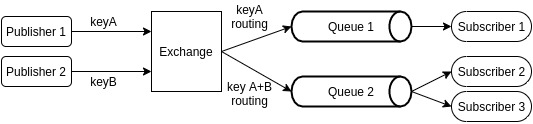
\includegraphics[width=1\textwidth,clip,trim=0 0 0 5]{Chapters/img/2_background/RabbitMQ.jpg}
    \caption{Publish/Subscribe example with RabbitMQ (adapted~\cite{rabbit-mq-pub-sub})} 
    \label{fig:rabbit-pubsub}
\end{figure}

Figure \ref{fig:rabbit-pubsub} represents a publish/subscribe scenario using RabbitMQ, composed of two publishers sending messages to a topic exchange, each having its respective key. Each subscriber is bound to a specific queue, and each queue is bound to the exchange using binding keys. Each queue can have several binding to an exchange, matching the subscribers particular interests. In this example, subscriber 1 receives messages that match type A while subscribers 2 and 3 will receive messages of type A and type B. 

\paragraph{\textbf{Kafka}} is an open-source distributed \gls{event-streaming} platform originally developed by LinkedIn. It was designed to collect and distribute high volumes of log data, as such it can be seen as both a log aggregator and a messaging system. 

Kafka is run as a cluster of one or more servers, some of which form the storage layer, called the \textbf{brokers} -- responsible for handling topics, store events and handle processing. While other servers run \textbf{Kafka Connect} to import and export data as even streams to integrate Kafka with existing systems such as \acrfull{rdbm}. 

Kafka starts with \textbf{events}, which record something that happened in the world or in the business. Everything written or read to Kafka is done in the form of events, which are composed of: a key, value, timestamp, and some optional data.

This events are published by client applications (\textbf{Producers}) to Kafka, and are then read and processed by subscribed \textbf{consumers}. Both, producers and consumers are fully decoupled and unaware of each other, which is one of the key elements for Kafka high scalability~\cite{6228206}. Servers and clients, communicate via high-performance custom TCP network protocol~\cite{custom-kafka-tcp-protocol}, which makes it harder to replace as its the only software using this protocol.

Unlike RabbitMQ that uses \acrshort{amqp}, Kafka does not implement the notion of a queue, instead events are organized and durably stored in \textbf{topics}. Each topic can have multiple subscribers and multiple producers. 

Events in a topic can be read as often as needed, as events are not deleted after consumption. Instead, it must be priorly established how long should events be retained through a per-topic configuration setting, after which old events are discarded. There is also flexibility on how to consume data, as the consumer controls the offset (position of records) whether by resetting to an older offset or by skipping ahead to the most recent one~\cite{10.1145/3242153.3242155}.  

Topics are \textbf{partitioned}, meaning a topic is spread over a number of groups located on different brokers~\cite{Kreps2011KafkaA}. Which allows clients to both read and write the data from/to many brokers at the same time. When a new event is published to a topic, it is appended to one of the topic's partitions. 

In Fig. \ref{fig:kafka-topic-partitions} it is possible to observe multiple consumers accessing partitions, some even simultaneously accessing different partitions, and accessing items in different offsets.

\begin{figure}[h]
    \centering
    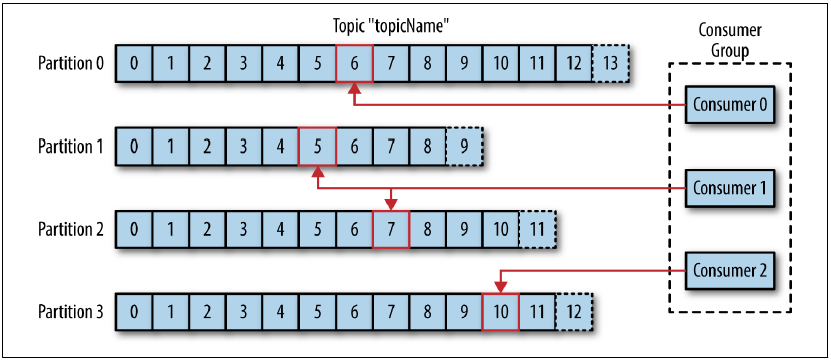
\includegraphics[width=1\textwidth,clip,trim=0 0 0 0]{Chapters/img/2_background/kafka-partitions.png}
    \caption{Topic with 4 partitions~\cite{kafka-partition-figure}} 
    \label{fig:kafka-topic-partitions}
\end{figure}

When published, events are appended to partitions using a round-robin distributing strategy to spread messages uniformly across partitions~\cite{Kreps2011KafkaA}. But events with the same key (e.g., estate id) are written to the same partition, and Kafka guarantees, by default, that any consumer of a given topic-partition will always read published events in the same order as they were written.

Data can be made fault-tolerant and highly available, by replicating every topic so that there are always multiple brokers with a copy of the data. However, Kafka really shines performance wise, while it may depend on external factors, such as design choices, it is capable of handling more than 100000 messages per second~\cite{kafka-thousand-requests} with the capability of reaching much higher values, without requiring state-of-the-art hardware~\cite{kafka-cheap-hardware}.

%Kafka uses Apache Zookeeper\footnote{\url{https://zookeeper.apache.org/}} as a coordination manager and failure recovery systems for brokers. Brokers are the nodes that handle topics, store events, and handle the processing.

%It does not use \acrshort{amqp}, as it does not implement the notion of a queue. Instead it stores collections of records in categories called \textbf{topics}. Each topic can have multiple subscribers assigned to it, and for each of these topics Kafka maintains a partitioned log of messages that can be located on different broker nodes in a Kafka cluster. Consumers control the offset (position of records) whether by a reset to an older offset or by skipping ahead to the most recent one, giving them flexibility on how to consume data.

%Kafka was explicitly designed to support less than a thousand topics~\cite{kafka-less-than-1000}. Each topic in Kafka is split into partitions that correspond to a logical log, each log consist of a set of segment files that all have approximately the same size. When a message is published to a topic and appended to partitions they are distributed using a round-robin partitioner to spread messages uniformly across partitions. 

%Kafka can be seen as a durable message broker where applications can process and re-process stream data on disk. Data is stored until a specified retention period has passed, meaning it is not removed once it is consumed. Instead, it can be replayed or consumed multiple times, if setup that way.

%Performance wise, while it may depend on external factors, such as design choices, Kafka is capable of handling more than 100000 messages per second~\cite{kafka-thousand-requests} with the capability of reaching much higher values, without requiring state-of-the-art hardware~\cite{kafka-cheap-hardware}.


% https://refubium.fu-berlin.de/bitstream/handle/fub188/29377/Thesis_HanWu.pdf?sequence=3&isAllowed=y

% Ver pagina 33 para mostrar um exemplo prático

\paragraph{\textbf{gRPC}} is a modern open source high performance \acrfull{rpc} framework that can run in any environment. A client application is able to directly call a method on a server application on a different machine as if it were a local object. As in many \acrshort{rpc} systems, gRPC is based around the idea of defining a service, specifying the methods that can be called remotely, and defining their parameters and return types. On the server side, the server implements this interface and runs a GRPC server to handle client calls. On the client side, there's a sub that provides the same methods as the server.

\begin{figure}[h]
    \centering
    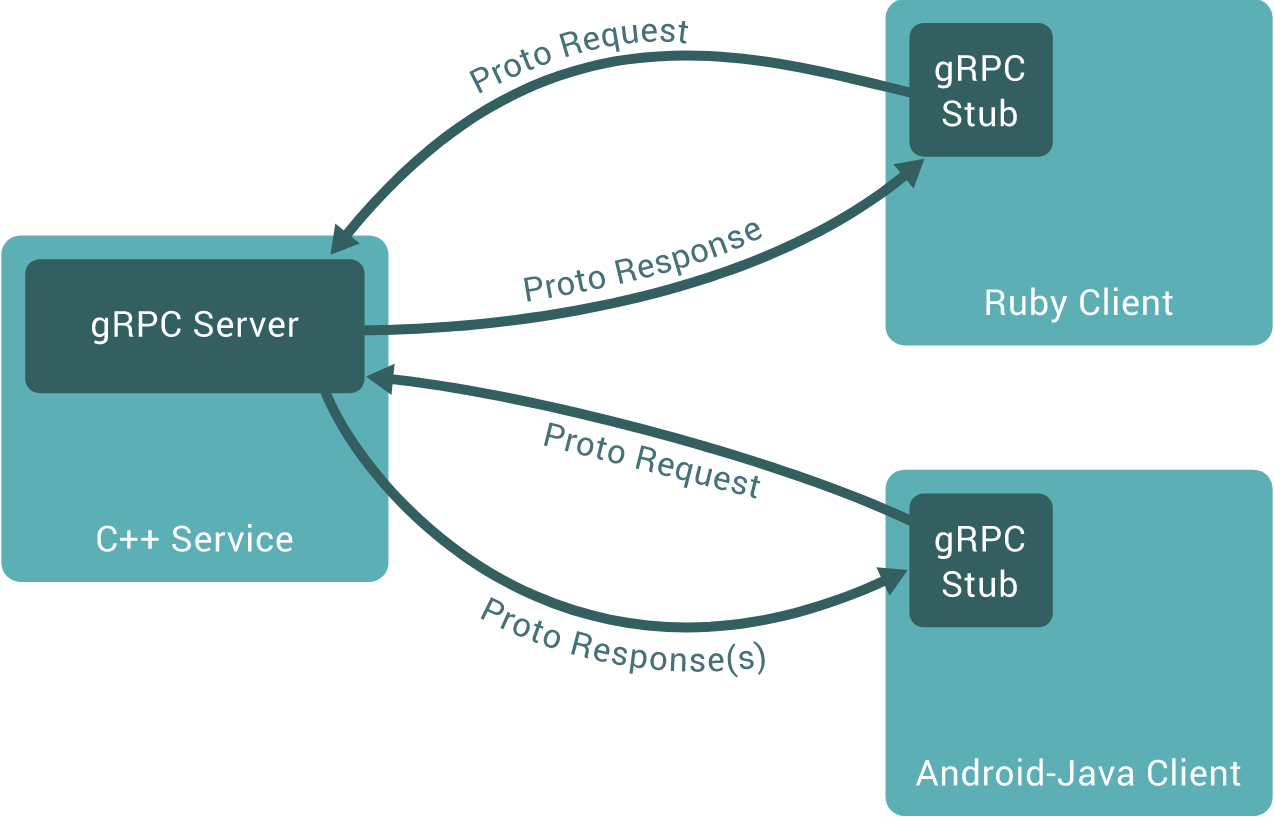
\includegraphics[width=0.75\textwidth,clip,trim=0 0 0 0]{Chapters/img/backend/gRPC.png}
    \caption{Client--Server example with gRPC~\cite{grpc-architecture-example}} 
    \label{fig:gprc-architecture-example}
\end{figure}

The clients and server can communicate between a variety of environments and languages. By default, it uses Protocol Buffers, Google's open source mechanism for serializing structured data, but also supports \acrshort{json}. To work with protocol buffers its required to define the structure of the data to be serialized in a \textit{proto file} (ordinary text file with a .proto extension). Protocol buffer data is structure as messages, where each message is a small logical record of information containing a series of name-value pairs called fields. Each field in the message has an unique number associated, these numbers are used to identify fields in the message binary format

\begin{lstlisting}
message IsochroneGrpc{
    int64 isochroneId = 1;
    string travelMode = 2;
}
\end{lstlisting}



Then, after specifying the data structures, it is necessary to use a protocol buffer compiler such as \textit{protoc} to generate data access classes in the language it will be used in. These provide CRUD like functions for each field such as \textit{setEstateId} and \textit{estateId}, as well as methods to serialize/parse the whole structure to/from raw bytes.

On top of messages, it is also necessary to define gRPC services in the proto files, where the method parameters and return types specified are protocol buffer messages.

\begin{lstlisting}
service IsochroneGrpcService{
    rpc getParamsInIsochroneGrpc(IsochroneGrpc) returns (ParamsGrpc);
}
\end{lstlisting}

gRPC offers a new take on the old RPC design by making it interoperable, modern, and efficient through the use of technologies such as Protocol Buffers and HTTP/2, some benefits:

\begin{itemize}
    \item \textbf{Lightweight messages}: depending on the type of call, gRPC-specific messages are usually much small than JSON messages;
    \item \textbf{High Performance} according to multiple evaluations, it is 5-10x times faster than REST+JSON communication;
    \item \textbf{Multiple parallel requests} due to HTTP/2 it supports multiple calls via the same channel and bidirectional communication -- a single connection can send both requests and responses at the same time;
    \item \textbf{Streaming} real-time communication, each stream is divided into frames that can be prioritized and run via a single TCP connection, thus reducing the network utilization and processing load.
\end{itemize}

% TODO Continuar https://grpc.io/docs/what-is-grpc/introduction/ & https://developers.google.com/protocol-buffers/docs/overview

\subsubsection{Storage}

As mentioned previously, according to the microservices guidelines each service should have its own storage solution. As such, we can pick a solution that perfectly fits the service it is destined for. The following technologies are the most popular DBMS in their respective models (Document, Wide-Column and Search engine), as of today~\cite{database-ranking}.

\paragraph{MongoDB} is a storage system written in C++ developed to handle issues related to scalability and agility~\cite{mongo-dev}. It is described as a free, open-source database with a flexible data structure, broad querying capabilities, and an architecture model that ensures scalability and high availability.

MongoDB's is a document-oriented database, composed of collections which are groups of MongoDB documents. A document is the basic structure for storing data it uses the \acrshort{bson} format that is made up of sets of \{key:value-pairs\}, and is required to have a unique identifier. Values can contain basic data types, arrays, and even objects.

One of the key points of MongoDB's data model is the lack of schema that specifies how documents should be structured within a collection. There are general guidelines to store documents of the same structure in one collection, but there is no enforcement for those rules. 
The second one is that the document structure enables hierarchical data through nesting capabilities, also due to its form, the model aligns well with object-oriented programming.

Finally, the model requires relations to be explicitly defined, either through subdocuments or referencing documents by their ids. Each method has advantages and disadvantages, but in general, subdocuments work better for small documents, while references are better for larger documents with dynamic data.

% Posso falar sobre sharding e replication se for importante
% https://ftp.utcluj.ro/pub/users/civan/IBD/3_EVALUARE/1_Referat/Resurse/B_2017_Mongo_cassandra.pdf
%MongoDB scalability comes from its implementation of sharding and replication, which allow it to distribute and duplicate data as necessary. 

\paragraph{AWS Dynamo} is a hosted NoSQL database offered by \acrfull{aws}, it was modelled after the principles of Dynamo~\cite{deCandia2007DynamoAH}, a database created by amazon in 2004-2007, when the company started to hit the upper scaling limits of its Oracle database.

The DynamoDB data model is composed of three core building blocks:

\begin{itemize}
    \item \textbf{Table} represents a grouping of data records, a similar concept to a table in PostgreSQL or a collection in MongoDB;
    \item \textbf{Item} is a single data record in a table, uniquely identified by the stated primary key of the table, equivalent to a document in MongoDB;
    \item \textbf{Attributes} are pieces of data related to a single item (e.g., height of a person). Unlike other PostgreSQL, DynamoDB does not require attributes on items except for attributes that make up a primary key.
\end{itemize}

Each item in a table is identified by a primary key, which must be defined at the creation of the table, and always provided when inserting a new item. There are two possible types for this key:

\begin{itemize}
    \item \textbf{Simple primary key} made up of just a partition key, similar to standard accessing rows in a SQL table through a primary key;
    \item \textbf{Composite primary key} which is composed of a partition key and a sort key, where sort keys are used to sort items with the same partition. An example could be an Orders table for recording customer orders on an e-commerce site, where the partition key would be the CustomerId, and the sort key would be the OrderId. 
\end{itemize}

However, querying items with primary keys is inefficient and as such, DynamoDB has the notion of secondary indexes. There are two main types: \textbf{local secondary indexes}, which uses the same partition key as the underlying table but a different sort key and \textbf{global secondary indexes}, which can define an entirely different primary key.

\paragraph{Elasticsearch}

Elasticsearch is a distributed, scalable, real-time search and analytics engine~\cite{elasticsearch-book}, built on top of Apache Lucene~\footnote{\url{https://lucene.apache.org/core/}}, a high-performance full-text search-engine library. Elasticsearch uses Lucene internally for all its indexing and searching, but makes it easier by abstracting the complexities of Lucene behind a RESTful API.

However, Elasticsearch adds much more functionality such as: distributed real-time document store where every field is indexed and searchable, a distributed search engine with real-time analytics and the capability to scale to hundreds of servers and petabytes of structured and unstructured data.

Underneath, it uses an inverted index which is term-centric, it organizes the information from a term to a list of documents which contain said terms, while the usual indexes are document-centric, as they map from documents to a list of terms. This list of documents are composed of integers, known as the document number. Each segment of an index is made up for a number of smaller files, where is what were considered the most important ones:

\begin{enumerate}
    \item \textbf{Field names}: field names used within the index;
    \item \textbf{Segment info}: Metadata about the segment, such as number of documents which it is based on;
    \item \textbf{Term dictionary}: All of the term occurrences in the indexed documents along with how many documents contain each term and a pointer to the frequency and proximity data for said term;
    \item \textbf{Term frequency data}: the document number of every which document that containers a term along with the number of occurrences of the term in said document;
    \item \textbf{Term proximity data}: The position(s) at which a term occurs in a document.
\end{enumerate}

Search results are returned based on their relevancy score, calculated with the use of Term Frequency/Inverse Document Frequency (TF/IDF)~\cite{8780663} scoring mechanism. When indexing or building queries this score can be manually increased or decreased to allow for more tailored results, but all turn off as well, meaning a document containing the search term several times will not be given preference over the one where it only occurs once. 

As the purpose of elastic search in this application is to match location names, where the number of occurrences is irrelevant, TF/IDF will not be a necessity. Normally, a match will only occur when the exact word used in the search query occurs in a document, but it can modified to allow fuzzy searches or to allow regular expressions to occurs in the search term. A fuzzy search allows matches to occur on phrases which vary slightly from the given search term, this level of fuzziness, can be automatically or manually configured. One change can be deleting, adding, changing a single character of switching the position of two adjacent characters. This type of solution makes the application more user friendly as it takes minor misspellings into account.

Any time that an instance of Elasticsearch starts, it is called a node. Every node in the cluster can handle \acrshort{http} and transport traffic. The transport layer is used exclusively for communication between nodes while the HTTP layer is used by REST clients. As the cluster grows, Elasticsearch allows the separation of relevant nodes to scale them as necessary, where are some of the most relevant nodes for this project:

\begin{itemize}
    \item \textbf{Master node} is responsible for lightweight cluster-wide actions such as creating and deleting indexes, tracking which nodes are part of the cluster, and deciding which shards to allocate to which nodes;
    \item \textbf{Data node} hold data and perform data-related operations such as CRUD, search, and aggregations;
    \item \textbf{Ingest node} are able to apply an ingest pipeline to a document to transform and enrich the document before indexing;
    \item \textbf{Coordination only} are responsible for routing requests, handle the search reduce phase, and distribute bulk indexing. In a way, acting as smart load balancers.
\end{itemize}

%%%%%%%%%%%%%%%%% TECNOLOGIAS DO CAPITULO USER INTERFACE

%%%%%%%%%%%%%%%%% TECNOLOGIAS DO CAPITULO MONITORING

%%%%%%%%%%%%%%%%% TECNOLOGIAS DO CAPITULO TESTING
